\documentclass[11pt]{amsart}
\usepackage[margin=1.1in]{geometry}
\usepackage{amsmath,amssymb,amsthm}
\usepackage{hyperref}
\usepackage{graphicx}
\newtheorem{theorem}{Theorem}
\newtheorem{proposition}[theorem]{Proposition}
\newtheorem{lemma}[theorem]{Lemma}
\theoremstyle{remark}
\newtheorem{remark}[theorem]{Remark}
\newcommand{\R}{\mathbb{R}}
\newcommand{\C}{\mathbb{C}}
\newcommand{\eps}{\varepsilon}
\newcommand{\ip}[2]{\langle #1,#2\rangle}
\newcommand{\re}{\operatorname{Re}}
\newcommand{\im}{\operatorname{Im}}

\title{Linear stability of the CDF shrinker $S_1$ modulo symmetries: a computer-assisted proof}
\author{Second supplement to the working notes for W.\,J.~Ogden and M.~Warren}
\date{November 5, 2026. Proof, code and draft by Claude (Anthropic) at M.~Warren's request.}

\begin{document}
\maketitle

\begin{abstract}
Let $S_1$ be the reflection-symmetric self-shrinker of curve diffusion flow constructed in the first supplement. We prove that, in the weighted space $L^2(e^{-\frac14(1+x^2)^{2/3}}dx)$, the linearization of the rescaled flow at $S_1$ has no eigenvalues with $\re\lambda>-\frac18$ other than the four produced by the symmetries: $\lambda=1$ (time shift) and $\lambda=\frac14$ (translation along the axis) for reflection-symmetric perturbations, and $\lambda=\frac14$ (translation across the axis) and $\lambda=0$ (rotation) for antisymmetric ones. Each is a simple zero of the Evans function of its class. The proof combines (i) semidefinite certificates for the numerical range, verified in ball arithmetic, which confine all eigenvalues with $\re\lambda\ge-\frac18$ to an explicit trapezoid; (ii) a Lyapunov--Perron construction of the admissible subspace at the conical end with explicit constants; and (iii) a validated computation, with CAPD, of the Evans functions along the boundary of the trapezoid, whose winding numbers are $2$ in each class.
\end{abstract}

\section{Statement}
Notation follows the first supplement: $\Gamma$ is parametrized by arclength $\sigma$ in the tail normalization ($q-\sigma\to0$ on the right end), $p=\ip{\Gamma}{\nu}$, $q=\ip{\Gamma}{T}$, $k$ the curvature, $m=k'$, and the profile system of the first supplement holds: $p'=-kq$, $q'=1+kp$, $k'=m$, $m'=p/4$. The tip is at $\sigma_{\rm tip}\in[-2.249127,-2.249019]$, and we write $x=\sigma-\sigma_{\rm tip}$ for arclength from the tip. The reflection symmetry gives $k,p$ even and $q,m$ odd in $x$.

A normal perturbation $\Gamma+u\nu$ of the rescaled flow $\partial_\tau\Gamma=(-k_{ss}+\frac14\ip{\Gamma}{\nu})\nu$ (modulo tangential reparametrization) evolves to first order by $\partial_\tau u=Lu$ with
\[
Lu=-u''''-k^2u''-(5kk'+\tfrac q4)u'+(\tfrac14-3k'^2-4kk'')u .
\]
(This was checked symbolically, \texttt{lincheck.py}.) One verifies directly $Lq=0$ (rotation), $Lp=p$ (time shift), and $L\ip{a}{\nu}=\frac14\ip{a}{\nu}$ for $a\in\R^2$ (translations). With $a$ along the symmetry line $\ell$, $\ip{a}{\nu}$ is even; across it, odd.

Let $\rho=e^{-\varphi}$, $\varphi=\beta(1+x^2)^{2/3}$, $\beta=\frac14$, and $H=L^2(\R,\rho\,dx)$. We call $\lambda\in\C$ an \emph{eigenvalue} if $Lu=\lambda u$ has a nontrivial smooth solution with $u^{(j)}\in H$ for $0\le j\le 4$. By the reflection symmetry every eigenfunction is a sum of an even and an odd one.

\begin{theorem}\label{thm:main}
Every eigenvalue of $L$ with $\re\lambda>-\frac18$ is one of
\begin{align*}
&\text{even class: }\ \lambda=1\ (u=p),\quad \lambda=\tfrac14\ (u=\ip{a_\parallel}{\nu});\\
&\text{odd class: }\ \ \lambda=\tfrac14\ (u=\ip{a_\perp}{\nu}),\quad \lambda=0\ (u=q).
\end{align*}
Each is a simple zero of the Evans function $D_{\rm even}$, respectively $D_{\rm odd}$, defined in \S\ref{sec:evans}. Moreover every eigenvalue with $\re\lambda\ge-\frac18$ satisfies
\[
\re\lambda\le1.7909,\qquad |\im\lambda|\le\frac{1.7683-\cos(0.48)\,\re\lambda}{\sin(0.48)}.
\]
\end{theorem}

\begin{remark}
Numerically (\texttt{evans.py} and \texttt{locate.py}), the even spectrum is $1$, $\frac14$, $-0.2561532$, $-0.6998896$, $-1.2151472$, $-1.6702734$, \dots\ and the odd spectrum is $\frac14$, $0$, $-0.4516348$, $-0.9663473$, $-1.4359417$, $-1.9260769$, \dots, all real. The theorem certifies the gap $\frac18$; the numerical gaps are $0.2562$ (even) and $0.4516$ (odd, beyond the rotation). For the hairpin problem only the even class matters, since curve diffusion flow preserves the reflection symmetry.
\end{remark}

\begin{figure}[h]
\centering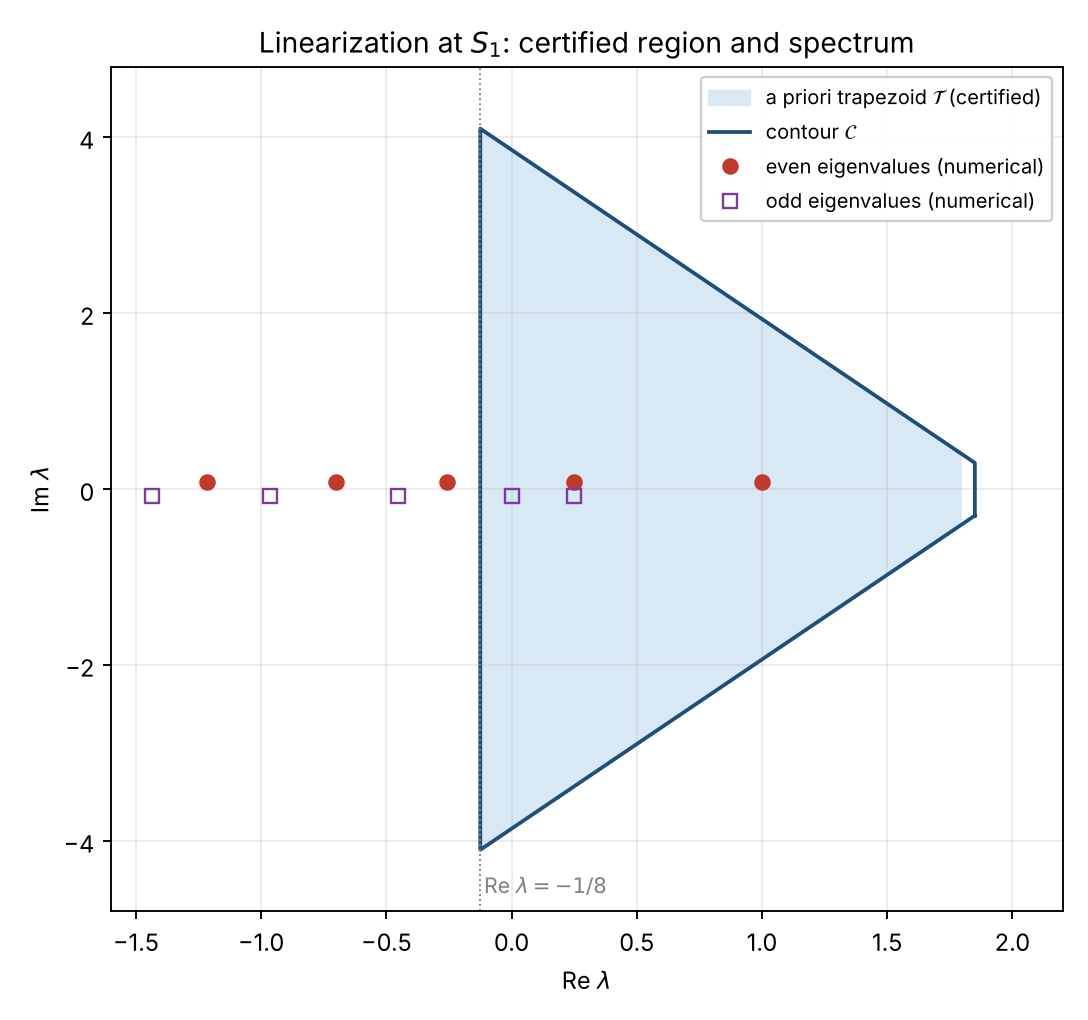
\includegraphics[width=0.62\textwidth]{spectrum_region.png}
\caption{The certified trapezoid $\mathcal T$ (Proposition~\ref{prop:apriori}), the contour $\mathcal C$, and the numerically computed eigenvalues (even: dots, odd: squares, offset vertically for visibility).}
\end{figure}

\section{A priori region: certificates for the numerical range}\label{sec:apriori}
Write $J=(u'',u',u)^T$. Two integrations by parts give, for every smooth $u$ with polynomial growth,
\[
\ip{Lu}{u}_H=\int_\R\Big(-|u''|^2+2\varphi'u''\bar u'-(g+k^2)u''\bar u+b\,u'\bar u+d\,|u|^2\Big)\rho\,dx,
\]
where $g=\varphi'^2-\varphi''$, $b=-(5km+\frac q4)$ and $d=\frac14-3m^2-kp$. Hence, for $\theta\in\R$, $\re(e^{i\theta}\ip{Lu}{u}_H)=\int J^*H_\theta J\,\rho$ with the Hermitian matrix
\[
H_\theta=\begin{pmatrix}-\cos\theta& e^{-i\theta}\varphi'& -e^{-i\theta}(g+k^2)/2\\ e^{i\theta}\varphi'&0& e^{-i\theta}b/2\\ -e^{i\theta}(g+k^2)/2& e^{i\theta}b/2&\cos\theta\, d\end{pmatrix}
\]
(entries $(i,j)$ multiply $\bar J_iJ_j$). For any $C^1$ Hermitian $2\times2$ matrix function $W=\begin{pmatrix}w_{11}&w_{12}\\ \bar w_{12}&w_{22}\end{pmatrix}$ the identity $\int(J_{\rm low}^*WJ_{\rm low}\,\rho)'\,dx=0$, $J_{\rm low}=(u',u)^T$, reads $\int J^*N_WJ\,\rho=0$ with
\[
N_W=\begin{pmatrix}0&w_{11}&w_{12}\\ w_{11}&w_{11}'+2\re w_{12}-\varphi'w_{11}&w_{12}'+w_{22}-\varphi'w_{12}\\ \bar w_{12}&\bar w_{12}'+w_{22}-\varphi'\bar w_{12}&w_{22}'-\varphi'w_{22}\end{pmatrix}.
\]
Consequently, if
\begin{equation}\label{eq:lmi}
P(x):=H_\theta(x)+N_W(x)-\Lambda E_{33}\preceq0\qquad\text{for all }x\in\R,
\end{equation}
then $\re(e^{i\theta}z)\le\Lambda$ for every $z$ in the numerical range of $L$ on such $u$, and in particular for every eigenvalue (eigenfunctions have polynomial growth, see \S\ref{sec:tail}, so all boundary terms vanish). This is the matrix (Legendre--Riccati) form of a sum-of-squares certificate; for large $|x|$ it reduces to the symbol inequality of the conjugated operator, which is sharp.

\emph{Construction.} We take $w_{11},w_{22}$ odd and $w_{12}=w_c+iw_d$ with $w_c,w_d$ even, as combinations of $x(1+x^2)^{-1/3}$, $x$, $(1+x^2)^{1/3}$, $1$ and symmetrized Gaussians $e^{-(x\mp c)^2/0.72}$ centred at $c=0,0.5,\dots,23.5$ ($48$ even, $47$ odd). Then $SP(-x)S=P(x)$ with $S=\mathrm{diag}(1,-1,1)$, so \eqref{eq:lmi} for $x\ge0$ implies it for all $x$. The coefficients are found by a semidefinite program on a grid, minimizing $\Lambda$ subject to $P\preceq-0.03\,I$ (\texttt{apr/sdp.py}, Clarabel). Two certificates are used:
\[
\theta=0:\ \Lambda_0=1.790819,\qquad \theta=0.48:\ \Lambda_1=1.768282 .
\]
For comparison, the suprema of the numerical range computed by discretization are about $1.73$ and $1.70$, so the certificates lose about $0.06$, the price of the margin.

\emph{Verification} (\texttt{apr/verify.py}, Arb ball arithmetic). On each $x$-box, the entries of $-P$ are enclosed, the midpoint matrix $M_c$ and the Frobenius norm $\varrho$ of the radii are formed, and Sylvester's criterion is checked for $M_c-\varrho I$; this implies $-P\succeq0$ on the box. The profile enters as follows:
\begin{enumerate}
\item[(1)] $x\in[0,\,8-\sigma_{\rm tip}]$: $30\,000$ CAPD enclosures of the solution curve of $S_1$ on the shooting bracket set (as in the first supplement, but finer), with the tip-time uncertainty added to the $x$-intervals; boxes are bisected in $x$ when needed ($29\,852$ checks).
\item[(2)] $\sigma\in[8,40]$: the bounds of the first supplement's tail proposition, $|k|,|k'|/\mu,|k''|/\mu^2\le\bar{\mathcal R}\,e^{-E(\sigma)}(8/\sigma)^{1/3}$, $q-\sigma=4kk'+4J$, $0\le J\le\bar{\mathcal R}^2(\frac\mu2+\frac1{12\sigma})e^{-2E}(8/\sigma)^{2/3}$ ($2104$, resp.\ $3160$, adaptive boxes).
\item[(3)] $x\ge X_v=40-\sigma_{\rm tip}$: with $u=x^{-1/3}$ and $D=\mathrm{diag}(u^{-2},u^{-1},1)$, the matrix $\hat P=u^4DPD$ is an explicit analytic function of $u\in[0,X_v^{-1/3}]$ (the Gaussian terms and the profile corrections are bounded by $3\cdot10^{-23}$). It is checked on $400$ $u$-intervals, including $u=0$.
\end{enumerate}
No box fails for either certificate. Since $L$ has real coefficients, the numerical range is invariant under conjugation, and the second certificate also gives $\cos(0.48)\re z+\sin(0.48)\im z\le\Lambda_1$.

\begin{proposition}\label{prop:apriori}
Every eigenvalue $\lambda$ with $\re\lambda\ge-\frac18$ lies in the closed trapezoid
\[
\mathcal T=\{-\tfrac18\le\re\lambda\le\Lambda_0,\ \ |\im\lambda|\le(\Lambda_1-\cos(0.48)\re\lambda)/\sin(0.48)\},
\]
whose height at $\re\lambda=-\frac18$ is $4.0694$ and at $\re\lambda=1.85$ is $0.2758$. In particular $\mathcal T$ lies strictly inside the contour $\mathcal C$ with vertices $1.85\pm0.3i$, $-0.125\pm4.1i$, except for its left edge, which lies on $\mathcal C$.
\end{proposition}

\section{The conical end}\label{sec:tail}
On $\sigma\ge\sigma_0=32$ write the eigenvalue equation as $u''''=a_2u''+a_1u'+a_0u$ with $a_0=c-3m^2-kp$, $c=\frac14-\lambda$, $a_1=-\frac\sigma4-5km-\frac{q-\sigma}4$, $a_2=-k^2$. Put $\mu=(\sigma/4)^{1/3}$, $\eps=c/\mu^4$, and let $\zeta_0,\dots,\zeta_3$ be the roots of $\zeta^4+\zeta=\eps$, continued from $0,-1,e^{\pm i\pi/3}$ at $\eps=0$. The \emph{G-pair} $\zeta_2,\zeta_3$ is enclosed by a Krawczyk test; the \emph{S-pair} enters only through $s=\zeta_0+\zeta_1=-(\zeta_2+\zeta_3)$ and $p_S=\zeta_0\zeta_1=-\eps/(\zeta_2\zeta_3)$, so a collision inside the S-pair is harmless. With $v(z)=(1,z,z^2,z^3)$, $e_+=\frac12(v(\zeta_0)+v(\zeta_1))=(1,\frac s2,\frac{s^2-2p_S}2,\frac{s^3-3sp_S}2)$, $e_-=\frac{v(\zeta_0)-v(\zeta_1)}{\zeta_0-\zeta_1}=(0,1,s,s^2-p_S)$ and $U=[e_+,e_-,v(\zeta_2),v(\zeta_3)]$, the substitution $Y=(u,u',u'',u''')^T=TZ$, $T=\mathrm{diag}(1,\mu,\mu^2,\mu^3)\,U\,\mathrm{diag}(1,\frac12,1,1)$, gives
\[
Z'=BZ,\qquad B=W_s^{-1}\Big[\mu\,\mathrm{blockdiag}\Big(\begin{pmatrix}\frac s2&1\\ \frac{s^2-4p_S}4&\frac s2\end{pmatrix},\zeta_2,\zeta_3\Big)-\frac{\widetilde M(\eps)}{3\sigma}+\mathcal P(\sigma)\Big]W_s,
\]
with $W_s=\mathrm{diag}(1,\frac12,1,1)$,
\[
\widetilde M=U^{-1}\mathrm{diag}(0,1,2,3)U-4\eps\,U^{-1}\partial_\eps U,\qquad
\mathcal P=U^{-1}e_4\Big(\frac{\delta a_0}{\mu^3},\frac{\delta a_1}{\mu^2},\frac{\delta a_2}{\mu},0\Big)U,
\]
the latter being the profile perturbation, bounded by the tail proposition. (The identities $U^{-1}A_\zeta U=\mathrm{blockdiag}(\cdots)$ and $T^{-1}T'=\widetilde M/(3\sigma)$ were also checked numerically, \texttt{check\_alg.py}.)

\begin{proposition}\label{prop:lp}
Let $\Lambda\subset\C$ be one of the boxes used below (side $0.074$ along $\mathcal C$, adaptive in the interior). For $\sigma\ge\sigma_0$ let $a(\sigma)\ge\|B_{GS}\|$, $b(\sigma)\ge\|B_{SG}\|$ and $g(\sigma)\le\lambda_{\min}(\mathrm{Herm}\,B_{GG})-\lambda_{\max}(\mathrm{Herm}\,B_{SS})$ for all $\lambda\in\Lambda$. If $g>0$, $(a+\eta^2b)/g\le\eta$ and $2\eta b/g<1$ on $[\sigma_0,\infty)$, then for each $\lambda\in\Lambda$ the set of solutions of polynomial growth is the graph $\{Z_G=\Gamma(\sigma)Z_S\}$ with $\sup\|\Gamma\|\le\eta$, $\Gamma(\sigma_0)$ is analytic in $\lambda$, and every other solution grows like $\exp((\frac a2-o(1))\sigma^{4/3})$, $a=\frac34 4^{-1/3}$, hence is not in $H$.
\end{proposition}

\begin{proof}[Sketch]
$\Gamma$ solves $\Gamma'=B_{GS}+B_{GG}\Gamma-\Gamma B_{SS}-\Gamma B_{SG}\Gamma$. The bounded solutions are the fixed points of $\Gamma(\sigma)=-\int_\sigma^\infty\Phi_G(\sigma,\tau)(B_{GS}-\Gamma B_{SG}\Gamma)\Phi_S(\tau,\sigma)\,d\tau$, and $\|\Phi_G(\sigma,\tau)\|\,\|\Phi_S(\tau,\sigma)\|\le e^{-\int_\sigma^\tau g}$ by the logarithmic-norm bounds. Then $\int_\sigma^\infty e^{-\int g}(a+\eta^2b)\le\sup\frac{a+\eta^2b}g\le\eta$, and the Lipschitz constant is at most $\sup2\eta b/g<1$. Analyticity follows from the uniform contraction. On the graph, $Z_S'=(B_{SS}+B_{SG}\Gamma)Z_S$ with logarithmic norm $O(1/\sigma)$, which gives polynomial growth. Off it, $\xi=Z_G-\Gamma Z_S$ satisfies $\xi'=(B_{GG}-\Gamma B_{SG})\xi$, so it grows at rate at least $g$; and since $g/\mu\to\frac12$ and $a>\beta$, such solutions are not in $H$.
\end{proof}

The bounds are computed in Arb on $120$ geometric $\sigma$-pieces of $[32,600]$, bisected where the bound is poor, plus an analytic final piece $[600,\infty)$ on which $a,b$ decrease and $g$ increases (\texttt{lin/lintail2.py}). On the $202$ boxes along $\mathcal C$ (side $0.074$), $\eta\le0.1163$ and $\sup 2\eta b/g\le0.272$.

\section{Evans functions}\label{sec:evans}
For $\lambda$ in a neighbourhood of $\mathcal T$, let $W(\sigma;\lambda)\in\Lambda^2\C^4$ solve the second-compound system with
\[
W(\sigma_0;\lambda)=\big(T[I;\Gamma(\sigma_0)]\big)_{\cdot 1}\wedge\big(T[I;\Gamma(\sigma_0)]\big)_{\cdot 2},
\]
which spans the admissible plane, and set $D_{\rm even}(\lambda)=W_{13}(\sigma_{\rm tip};\lambda)$ and $D_{\rm odd}(\lambda)=W_{02}(\sigma_{\rm tip};\lambda)$ (coordinates $(u,u',u'',u''')$). These are analytic on a neighbourhood of $\mathcal T$, by the interior cover of \S\ref{sec:winding}, and $D(\bar\lambda)=\overline{D(\lambda)}$. An even eigenfunction restricts to an admissible solution with $u'=u'''=0$ at the tip, and conversely; the plane meets $\{u'=u'''=0\}$ nontrivially iff $W_{13}=0$. Likewise for odd functions with $u=u''=0$ and $W_{02}$. So the zeros of $D_{\rm even}$ ($D_{\rm odd}$) in $\mathcal T$ are exactly the even (odd) eigenvalues.

\section{Winding numbers}\label{sec:winding}
By the symmetry $D(\bar\lambda)=\overline{D(\lambda)}$ and the reality of $D$ on $\R$, the winding number of $D$ along $\mathcal C$ equals $\frac1\pi$ times the change of $\arg D$ along the upper half $1.85\to1.85+0.3i\to-0.125+4.1i\to-0.125$.

\emph{Enclosures} (\texttt{cap/evans\_seg.cpp}, \texttt{cap/seg2.py}, \texttt{cap/contour.py}). The upper half is split into $N=5058$ segments $[\lambda_a,\lambda_b]$ of length between $10^{-4}$ and $0.004$ (chosen from $\eta$ and refined adaptively). For each segment we introduce $t\in[0,1]$ with $\lambda=\lambda_a+t(\lambda_b-\lambda_a)$ as a state variable, so that CAPD tracks the dependence on $\lambda$ linearly, and integrate the $17$-dimensional system for $(p,q,k,m)$, $W$ and $t$:
\begin{enumerate}
\item[(B)] from $\sigma=32$ to $8$. The initial plane is $T[I;\Gamma]$ with $\Gamma$ in the $\eta$-ball as $8$ parameter columns, $\det\Gamma\,(T_G)_{\cdot1}\wedge(T_G)_{\cdot2}$ as $2$ more, and the $t$-dependence via $\partial_\lambda T$ with a mean-value remainder. The profile box at $\sigma=32$ comes from the tail proposition. Fixed steps $h=\min(0.1,3.2/\sigma)$ are used, and the profile and $W$ are rescaled by powers of two every $8$ units.
\item[(C)] from $\sigma=8$ to the tip. The tight shooting-bracket set of the first supplement is used for the profile, and the $W$- and $t$-rows of the stage-B set are carried over. The fixed time $\tau=10.249019$ is followed by the window $[10.249019,10.249127]$ that contains the tip time of $S_1$.
\end{enumerate}
The output is an affine enclosure $D(\lambda_a+t(\lambda_b-\lambda_a))\in X+V(t-\frac12)+E$, with $E$ a complex box, for both classes. We check rigorously that $0\notin S_i:=X+V[-\frac12,\frac12]+E$, which is convex, and choose $\alpha_i$ in the intersection of the end box of segment $i-1$ and the start box of segment $i$. Both boxes contain $D(\lambda_i)$, so $\alpha_i\in S_{i-1}\cap S_i$. Then $\sum_i\mathrm{pv}\arg(\alpha_{i+1}/\alpha_i)$ equals the exact change of $\arg D$, because consecutive representatives lie in a common convex set avoiding $0$. Inside CAPD, $W$ is multiplied on each segment by positive powers of two, so $S_i$ encloses $c_iD$ for some $c_i>0$. We therefore use the convex cones $K_i=\R_{>0}S_i$, which avoid $0$ and contain $D(\text{segment }i)$. We take $\alpha_i$ on a ray in the intersection of the argument intervals of the end box of segment $i-1$ and the start box of segment $i$ (\texttt{cap/winding\_cert.py}), and the statement above holds with $K_i$ in place of $S_i$. At the two real endpoints $\alpha=\pm1$. There $D_{\rm even}$ and $D_{\rm odd}$ are both negative: at $1.85$ the boxes are $-0.01936\pm10^{-4}$ and $-0.02957\pm10^{-4}$ in the scaled units, and at $-\frac18$ they are $-4.39\cdot10^{-6}\pm4\cdot10^{-8}$ and $-1.79\cdot10^{-6}\pm1.3\cdot10^{-8}$.

\emph{Result.} The change of $\arg D_{\rm even}$ along the upper half is $2\pi$, and so is that of $\arg D_{\rm odd}$. Both winding numbers along $\mathcal C$ are therefore $2$. The largest step $|\mathrm{pv}\arg(\alpha_{i+1}/\alpha_i)|$ is $0.33$. The ratio $|E|/\mathrm{dist}(0,X+V[-\frac12,\frac12])$ has median $0.53$; every segment passes the rigorous test that it is $<1$.

\emph{Analyticity inside $\mathcal C$} (\texttt{cap/interior.py}). The hypotheses of Proposition~\ref{prop:lp} hold on $174$ boxes of side $0.2$ or $0.1$, each enlarged by $0.01$, covering a neighbourhood of the closed upper half of the region bounded by $\mathcal C$, with $\eta\le0.262$ and $\sup2\eta b/g\le0.931$. All bounds are invariant under $\lambda\mapsto\bar\lambda$, so this also covers the lower half. On overlaps the graphs agree by uniqueness of the bounded solution, so $\Gamma(\sigma_0;\lambda)$, and hence $D_{\rm even}$ and $D_{\rm odd}$, are analytic on a neighbourhood of the closed region.

\begin{proof}[Proof of Theorem~\ref{thm:main}]
By Proposition~\ref{prop:apriori}, every eigenvalue with $\re\lambda>-\frac18$ lies in the interior of $\mathcal C$, and none lies on the left edge, since $0\notin S_i$ there. By \S\ref{sec:evans} these are the zeros of $D_{\rm even}$, $D_{\rm odd}$, which are analytic inside $\mathcal C$. Each winding number is $2$. The listed symmetry eigenvalues are zeros of the respective functions, with eigenfunctions $p,\ip{a_\parallel}{\nu}$ (even) and $\ip{a_\perp}{\nu},q$ (odd), so they are all the zeros and each is simple. The a priori bounds are Proposition~\ref{prop:apriori}.
\end{proof}

\begin{remark}[Multiplicity]
For Evans functions built from bases of the admissible subspaces that are analytic in $\lambda$, the order of a zero equals the algebraic multiplicity of the eigenvalue (Gardner--Jones; see Kapitula--Promislow, \emph{Spectral and dynamical stability of nonlinear waves}, Ch.~9). Applied here, the four eigenvalues are algebraically simple within their classes. We have not written out the verification of the hypotheses of that theorem in this half-line, weighted setting; this is the one place where the argument relies on a standard result rather than a check done here.
\end{remark}

\section{Reproducibility and trust base}
All rigorous steps rerun with CAPD~6.1.0 and python-flint~0.9. The trust base is CAPD's interval ODE solver, Arb's ball arithmetic, the first supplement (profile enclosures and tail bounds), and the hand arguments in Propositions~\ref{prop:apriori} and~\ref{prop:lp}. The SDP solver is not part of the trust base: its output is only a candidate, which is then verified.

What remains toward Conjecture~7.1: step 3 (nonlinear stability of $S_1$ in the symmetric class, modulating the time-shift and axial-translation modes, with explicit constants) and step 4 (validated integration of an embedded hairpin into that basin).
\end{document}
